\documentclass{article}
\usepackage{amsfonts} % if you want blackboard bold symbols e.g. for real numbers
\usepackage{graphicx} % if you want to include jpeg or pdf pictures
\usepackage{amsmath}
\usepackage{chngcntr}
\usepackage{wrapfig}
\usepackage{caption}
\usepackage{subcaption}
\usepackage[utf8]{inputenc}
\usepackage[latin1]{inputenc}
\usepackage[francais]{babel}


\title{Le Guide du Programmeur}
\author{Nom Prenom }
\date{December 2015}

\usepackage{natbib}
\usepackage{graphicx}

\begin{document}

\maketitle

\section{Introduction}

There is a theory which states that if ever anyone discovers exactly what the Universe is for and why it is here, it will instantly disappear and be replaced by something even more bizarre and inexplicable.
There is another theory which states that this has already happened.

\begin{figure}[h!]
\centering
\includegraphics[scale=1.7]{universe.jpg}
\caption{The Universe}
\label{fig:univerise}
\end{figure}

\section{Architecture globale et Page d'accueil}

L'architecture du site web est découpée en trois grande partie

\begin{itemize}
\item[$\bullet$] La page d'accueil est dans le dossier 'src'
\item[$\bullet$] Les formulaires d'inscription sont dans 'src/inscription'
\item[$\bullet$] L'interface staff est dans 'src/staff'
\end{itemize}\\

Langages utilisés
\begin{itemize}
\item[$\bullet$] Côté Client: \begin{itemize}
        \item[$\bullet$] HTML
        \item[$\bullet$] CSS
        \item[$\bullet$] Javascript
    \end{itemize}
\item[$\bullet$] Côté Serveur: \begin{itemize}
        \item[$\bullet$] PHP
        \item[$\bullet$] MySQL
    \end{itemize}
\end{itemize}\\

Framework utilisés
\begin{itemize}
\item[$\bullet$] CSS: \begin{itemize}
        \item[$\bullet$] Bootstrap
        \item[$\bullet$] Font-Awesome
    \end{itemize}
\item[$\bullet$] JS: \begin{itemize}
        \item[$\bullet$] Bootstrap
        \item[$\bullet$] Datatable
        \item[$\bullet$] jquery
    \end{itemize}
\end{itemize}\\
La page d'accueil est directement située dans le dossier 'src' et correspond au fichier 'src/index.php'.

\begin{figure}[h!]
\centering
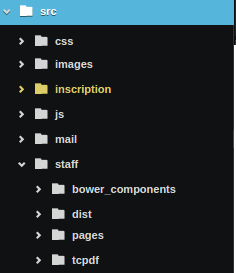
\includegraphics[scale=0.7]{Structure.png}
\caption{Arborescence de l'application}
\end{figure}


\section{Page d'accueil}

\begin{itemize}
\item[$\bullet$] Lien : src/index.php
\item[$\bullet$] Style : 'src/css'
\item[$\bullet$] JS : 'src/js'
\item[$\bullet$] Images 'src/images'
\end{itemize}

Le framework css utilisé bootstrap (bootstrap.min.css), et le template style.css\\
Le css personnalisés sont et monStyle.css\\
\begin{figure}[h!]
\centering
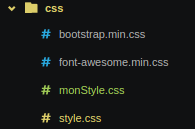
\includegraphics[scale=1]{CSSAccueil.png}
\caption{Styles utilisés pour la page d'accueil utilisateur}
\end{figure}

\\
Les frameworks javascript utilisés sont bootstrap, jquery, jqBootstrapValidation.js, html5shiv.js
et le template script.js\\
\begin{figure}[h!]
\centering
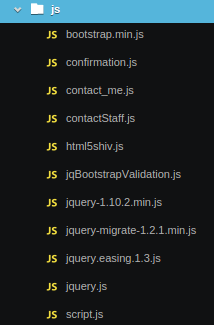
\includegraphics[scale=1]{JSAccueil.png}
\caption{Scripts utilisés pour la page d'accueil utilisateur}
\end{figure}

Les fichiers contact\_me.js, contactStaff.js sont les fichiers permettant de faire fonctionner l'envoie de mail via la page d'accueil.\\
\begin{figure}[h!]
\centering
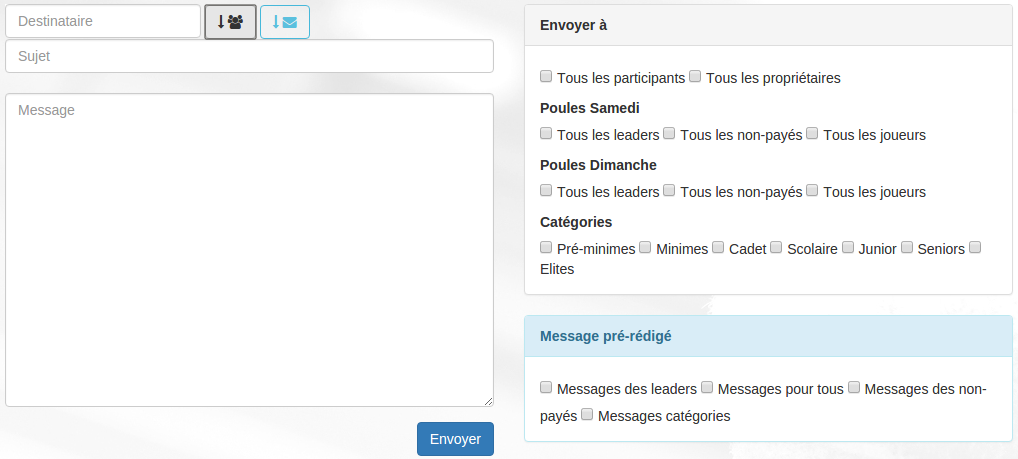
\includegraphics[scale=1]{mailAccueil.png}
\caption{Interface pour envoie du mail au staff}
\end{figure}

\section{Inscription Joueurs \& Propriétaire}
Les formulaires d'inscription pour les joueurs et les propriétaires sont situés dans le dossier 'src/inscription'. Ce sont les formulaires que les visiteurs utiliseront pour s'inscrire.\\
Le formulaire d'inscription de joueurs correspond au fichier 'src/inscription/index.php'.\\
Le formulaire d'inscription de joueurs correspond au fichier 'src/inscription/inscription-owner.php'.\\

\begin{figure}[h!]
\centering
\includegraphics[scale=0,7]{arboInsccription.png}
\caption{Arborescence pour les inscriptions côté utilisateur}
\end{figure}


\section{Interface Staff}

\subsection{Présentation}

\begin{itemize}
\item[$\bullet$] Lien : src/staff/pages
\item[$\bullet$] Librairies/Dépendances : src/staff/bower\_components
\item[$\bullet$] Style : 'src/staff/dist/css'
\item[$\bullet$] JS : 'src/staff/dist/js'
\item[$\bullet$] Outil génération PDF : 'src/staff/tcpdf'
\end{itemize}

Les librairies Bootstrap, font-awesome, et datatables ont été essentiellement utilisées.
Les css personnalisés sont dans dist/

\subsection{Ajout, Edition et Liste}

Fichiers php dans le dossier src/staff/pages/ –> pages affichées dans l'application

Fichiers php dans le dossier src/staff/pages/php –> pages appelées par des methodes get/post pour faire du traitement de la base de donnée.

Fichiers inc dans le dossier src/staff/pages/php/inc -> fonctions pour avoir un code plus découpé

Le dossier 'src/staff/pages' contient tous les formulaires (ou vues) d'ajout et d'édition des entités (joueur, propriétaire, terrain, match, …). Ils sont représentés par des fichier PHP. Les formulaires d'édition sont caractérisés par le mot 'edit' en début de nom de fichier. Les formulaires d'ajout sont simplement désignés par le nom de l'entité qui leur correspond. Par exemple, le fichier 'court.php' correspond au formulaire d'ajout un terrain, et le fichier 'edit-court.php' correspond au formulaire d'édition d'un terrain.

Le dossier 'html' contient un fichier 'header.php' qui correspond à l'en-tête visible sur toutes les pages de l'interface Staff.

Le dossier 'php' contient toutes les fonctions d'interaction avec la base de données. Les fonctions d'ajout sont situées dans les fichiers dont le nom commence par 'add'. Les fonctions de suppression sont situées dans les fichiers dont le nom commence par 'delete'.
Le dossier 'inc' (dans 'php') contient les fonctions d'affichage et d'édition. Les fonctions d'édition sont situées dans les fichiers dont le nom commence par 'edit'. Les fonctions d'affichage sont situées dans les fichiers dont le nom commence par 'list' (pour les listes) et 'show' (pour les affichages unitaires).


\subsubsection{Vues}

Toutes les pages affichées se trouvent dans le dossier src/staff/pages/

Le dossier 'html' contient un fichier 'header.php' qui correspond à l'en-tête visible sur toutes les pages de l'interface Staff.

% \begin{figure}[h!]
% \centering
% \includegraphics[scale=1]{arboList.png}
% \caption{Exemple d'un tableau d'affichage list.php}
% \end{figure}

\begin{figure}[h!]
\centering
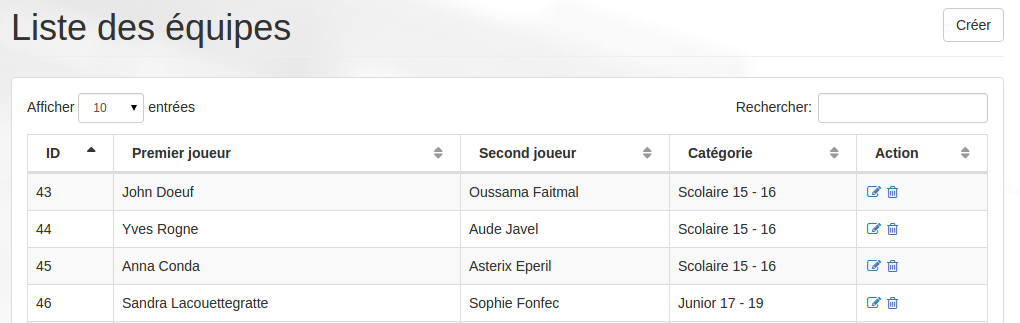
\includegraphics[scale=0.7]{tableau.png}
\caption{Exemple d'un tableau d'affichage list.php}
\end{figure}

\begin{figure}[h!]
\centering
\includegraphics[scale=0.7]{show.png}
\caption{Exemple d'une vue sur les détails (show.php)}
\end{figure}

\begin{figure}[h!]
\centering
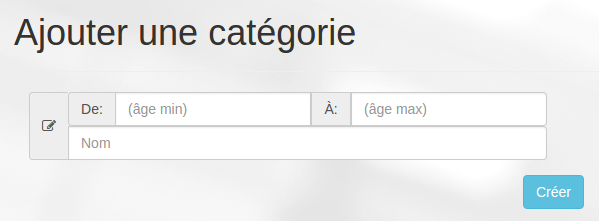
\includegraphics[scale=0.7]{form.png}
\caption{Exemple d'une vue sur un ajout (player.php, owner.php...)}
\end{figure}

\begin{itemize}
\item[$\bullet$]{\textbf{Participant: }}
\begin{tabular}{ccc}
 Ajout & Edition & Affichage \\
 \hline
player.php & edit-player.php & list.php?=player\\
  &  & show.php?=player
\end{tabular}

\item[$\bullet$]{\textbf{Equipe: }}
\begin{tabular}{ccc}
 Ajout & Edition & Affichage \\
 \hline
team.php & edit-team.php & list-team.php\\
  & show-team.php
\end{tabular}

\item[$\bullet$]{\textbf{Match: }}
\begin{tabular}{ccc}
 Ajout & Edition & Affichage \\
 \hline
match.php & edit-match.php & list-match.php\\
  & & show-match.php
\end{tabular}

\item[$\bullet$]{\textbf{Catégorie: }}
\begin{tabular}{ccc}
 Ajout & Edition & Affichage \\
 \hline
category.php & edit-category.php & list.php?=category\\
  &  & show.php?=category
\end{tabular}

\item[$\bullet$]{\textbf{Propriétaire: }
\begin{tabular}{ccc}
 Ajout & Edition & Affichage \\
 \hline
owner.php & edit-owner.php & list.php?=owner\\
  &  & show.php?=owner
\end{tabular}

\item[$\bullet$]{\textbf{Terrain: }
\begin{tabular}{ccc}
 Ajout & Edition & Affichage \\
 \hline
court.php & edit-court.php & list.php?=court\\
  &  & show.php?=court
\end{tabular}

\item[$\bullet$]{\textbf{Staff: }
\begin{tabular}{ccc}
 Ajout & Edition & Affichage \\
 \hline
- & - & list.php?=court\\
  &  & show.php?=court
\end{tabular}

\item[$\bullet$]{\textbf{Extra: }}
\begin{tabular}{ccc}
 Ajout & Edition & Affichage \\
 \hline
extra.php & edit-extra.php & list-extras.php\\
  &  & show.php?=extra
\end{tabular}

\end{itemize}



\subsubsection{Modification de la Base de Données}
Toutes les modifications de la base de donnée affichées se trouvent dans le dossier src/staff/pages/php

\begin{figure}[h]

\begin{subfigure}{0.5\textwidth}
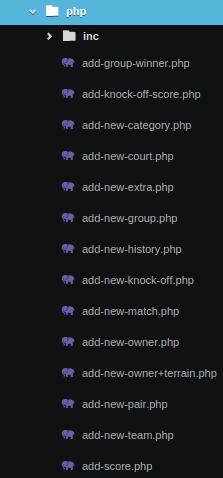
\includegraphics[\linewidth, height=5cm]{arboAdd.png}
\caption{Caption1}
\label{fig:subim1}
\end{subfigure}
\begin{subfigure}{0.5\textwidth}
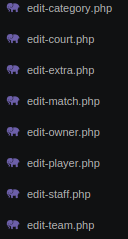
\includegraphics[\linewidth, height=5cm]{arboEdit.png}
\caption{Caption 2}
\label{fig:subim2}
\end{subfigure}

\caption{Caption for this figure with two images}
\label{fig:image2}
\end{figure}

\begin{figure}[h!]
\centering
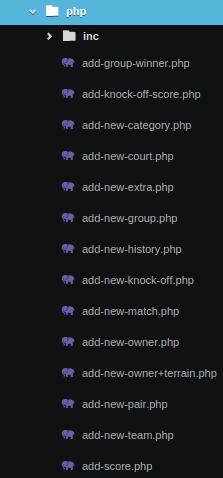
\includegraphics[scale=0.7]{arboAdd.png}
\caption{Fichiers d'ajout à la BDD}
\end{figure}

\begin{figure}[h!]
\centering
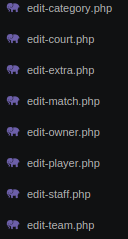
\includegraphics[scale=0.7]{arboEdit.png}
\caption{Fichiers d'édition de la BDD}
\end{figure}

\begin{figure}[h!]
\centering
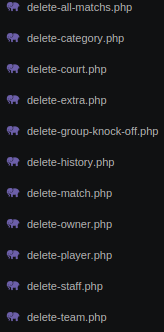
\includegraphics[scale=0.7]{arboDelete.png}
\caption{Fichiers de suppression de la BDD}
\end{figure}

\begin{itemize}
\item[$\bullet$]{\textbf{Participant: }}
\begin{tabular}{ccc}
 Ajout & Edition & Suppresion \\
 \hline
add-new-pair.php & edit-player.php & delete-player.php\\
\end{tabular}

\item[$\bullet$]{\textbf{Equipe: }}
\begin{tabular}{ccc}
 Ajout & Edition & Suppresion \\
 \hline
add-new-team.php & edit-team.php & delete-team.php\\
\end{tabular}

\item[$\bullet$]{\textbf{Match: }}
\begin{tabular}{ccc}
 Ajout & Edition & Suppresion \\
 \hline
add-new-match.php & edit-match.php & delete-match.php\\
\end{tabular}

\item[$\bullet$]{\textbf{Catégorie: }}
\begin{tabular}{ccc}
 Ajout & Edition & Suppresion \\
 \hline
add-new-category.php & edit-category.php & delete-category.php\\
\end{tabular}

\item[$\bullet$]{\textbf{Propriétaire: }
\begin{tabular}{ccc}
 Ajout & Edition & Suppresion \\
 \hline
add-new-owner.php & edit-owner.php & delete-owner.php\\
\end{tabular}

\item[$\bullet$]{\textbf{Terrain: }
\begin{tabular}{ccc}
 Ajout & Edition & Suppresion \\
 \hline
add-new-court.php & edit-court.php & delete-court.php\\
\end{tabular}

\item[$\bullet$]{\textbf{Staff:}
\begin{tabular}{ccc}
 Ajout & Edition & Suppresion \\
 \hline
- & - & - \\
\end{tabular}

\item[$\bullet$]{\textbf{Extra: }
\begin{tabular}{ccc}
 Ajout & Edition & Suppresion \\
 \hline
add-new-extra.php & edit-extra.php & delete-extra.php\\
\end{tabular}

\end{itemize}

\subsubsection{Fichiers .inc}
Les fichiers inc se trouvent dans le dossier src/staff/pages/php/inc
fonctions pour avoir un code plus découpé

\begin{figure}[h!]
\centering
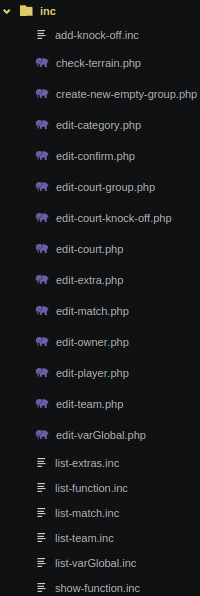
\includegraphics[scale=0.7]{arboInc.png}
\caption{}
\end{figure}

\subsection{Poules}

\subsubsection{Vues}

\begin{figure}[h!]
\centering
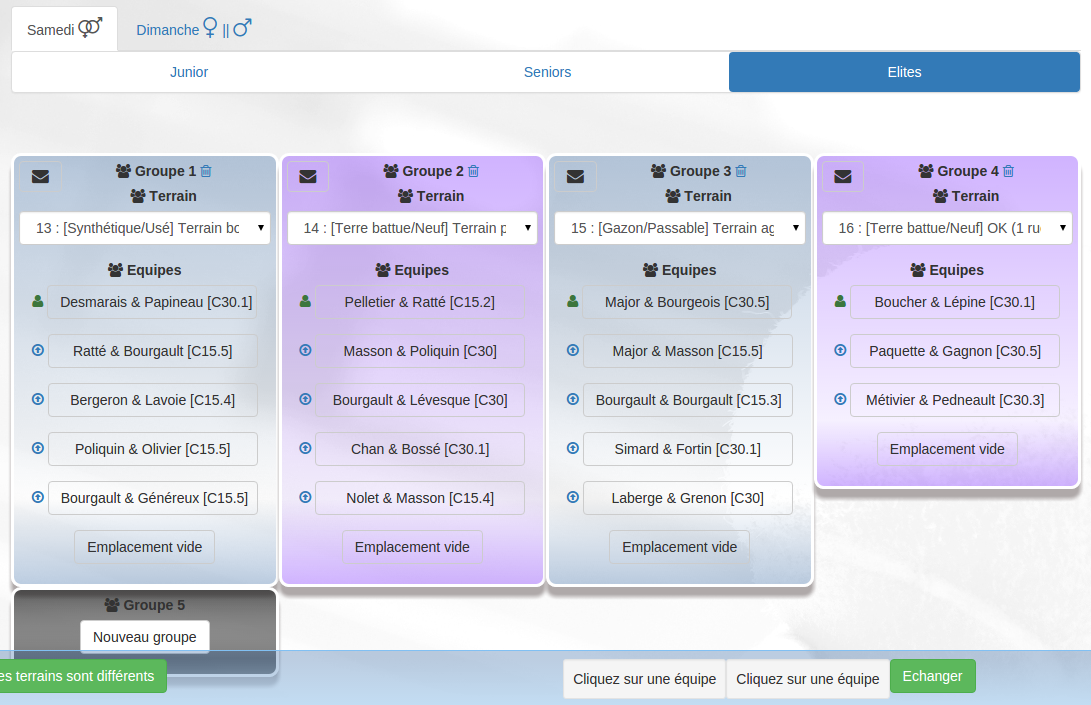
\includegraphics[scale=0.7]{group.png}
\caption{}
\end{figure}

\subsubsection{Modification de la Base de données}


\subsection{Knock-off}

\subsubsection{Vues}

\begin{figure}[h!]
\centering
\includegraphics[scale=0.7]{knockoff.png}
\caption{}
\end{figure}

\subsubsection{Modification de la Base de données}


\section{Structure de la Base de données}
La Base de données utilisées est en MySQL

\begin{figure}[h!]
\centering
\includegraphics[scale=0.7]{diagramme.png}
\caption{}
\end{figure}

\begin{figure}[h!]
\centering
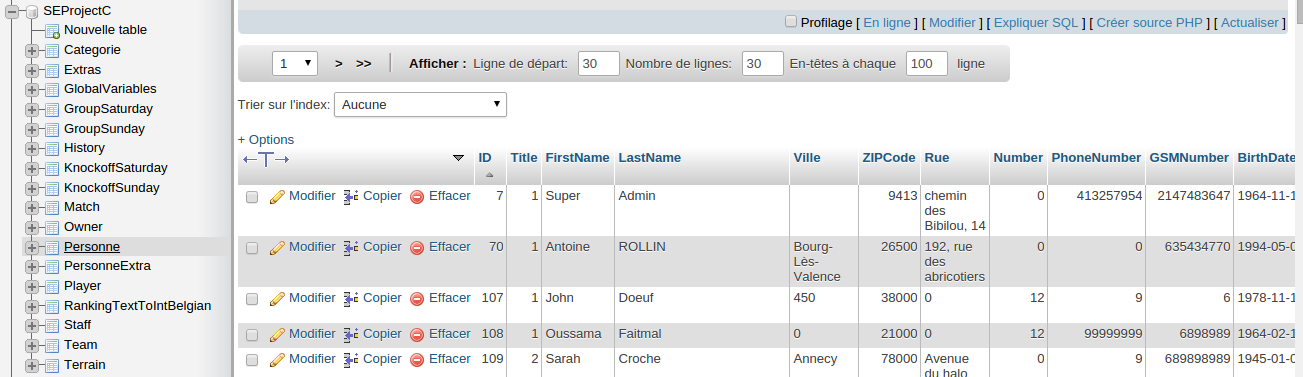
\includegraphics[scale=0.7]{phpMyAdmin.png}
\caption{}
\end{figure}

La  base  de  données  est  de  type SQL. Elle  correspond  au  fichier  de  format  ‘.sql’  dans  le dossier ‘docs’.

La  base  de  données  contient  les  différentes  tables  nécessaires  au  fonctionnement  de l’application :

\begin{itemize}
\item[$\bullet$]{\textbf{Categorie :}} contient les différentes catégories possibles (une catégorie est attribuée
 à une équipe en fonction de l’âge du plus vieux des membres)

\item[$\bullet$]{\textbf{Extras :}} contient les extras (activités annexes proposées au joueurs)

\item[$\bullet$]{\textbf{GlobalVariables :}} contient différentes variables (telles que les contenus de mail ou le prix du tournoi)

\item[$\bullet$]{\textbf{GroupSaturday :}} contient les poules pour le samedi

\item[$\bullet$]{\textbf{GroupSunday :}} contient les poules pour le dimanche

\item[$\bullet$]{\textbf{History  :}}  contient  toutes  les  modifications  apportées  à  la  base  de  données (ajout, édition, suppression)

\item[$\bullet$]{\textbf{KnockoffSaturday :}} contient tous les matchs de Knock-Off du samedi (liée à la table Match)

\item[$\bullet$]{\textbf{KnockoffSunday  :}}  contient  tous  les  matchs  de  Knock-Off  du  dimanche  (liée  à  la table Match)

\item[$\bullet$]{\textbf{Match :}} contient tous les matchs du tournoi

\item[$\bullet$]{\textbf{Owner :}} contient toutes les informations relatives aux propriétaires inscrits (liée à la table Personne)

\item[$\bullet$]{\textbf{Personne  :}}  contient  toutes  les  informations  relatives  aux  personnes  inscrites (joueurs, propriétaires, staff)

\item[$\bullet$]{\textbf{PersonneExtra :}} contient les choix d’extras des joueurs (liée à la table Personne)

\item[$\bullet$]{\textbf{Player :}} contient toutes les informations relatives aux joueurs inscrits

\item[$\bullet$]{\textbf{RankingTextToIntBelgian :}} contient tous les rangs officiels possibles pour un joueur classé

\item[$\bullet$]{\textbf{Staff  :}}  contient  toutes  les  informations  relatives  aux  membres  du  staff  enregistrés (liée à la table Personne)

\item[$\bullet$]{\textbf{Team :}} contient toutes les équipes inscrites

\item[$\bullet$]{\textbf{Terrain :}} contient tous les terrains enregistrés (liée à la table Owner)
\end{itemize}


\section{Test}
\subsection{Ghost Inspector}

Logiciel payant limité à 100 test par mois. Facilité de générer des scripts\\
\begin{figure}[h!]
\centering
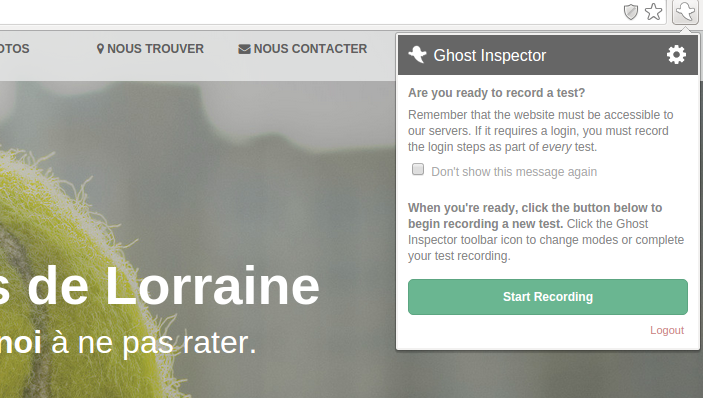
\includegraphics[scale=0.7]{ghost.png}
\caption{Démarrer une simulation}
\end{figure}

\begin{figure}[h!]
\centering
\includegraphics[scale=0.7]{ghostInterface.png}
\caption{Gérer ses tests}
\end{figure}

\subsection{Selenium}

Executer un script\\
\begin{figure}[h!]
\centering
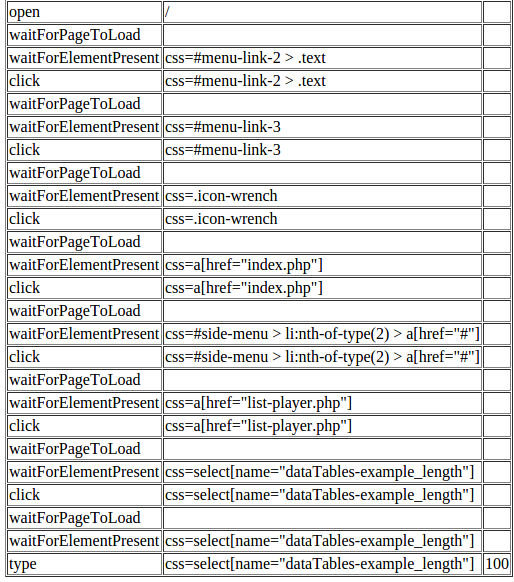
\includegraphics[scale=0.7]{selenium.png}
\caption{}
\end{figure}

\section{Conclusion}
``I always thought something was fundamentally wrong with the universe'' \citep{adams1995hitchhiker}

\bibliographystyle{plain}
\bibliography{references}

\end{document}
